\documentclass[../main.tex]{subfiles}

\begin{document}
\قسمت{آقای یا خانم؟}

\زیرقسمت{مقدمه}
\پاراگراف{}
یکی از سخترین کارها در کلاس و مخصوصا کلاس‌های آنلاین استفاده صحیح از پیشوندهای آقای و خانم است.
مثلا شما در لیست اسم پرهام الوانی را می‌بینید و نمی‌دانید باید بگویید آقای الوانی یا خانم الوانی.
در این تمرین قصد داریم وب‌سایتی طراحی کنیم که در این امر مهم اساتید را یاری دهد.
در این سایت دو حالت کلی وجود دارد زمانی که کاربر از جنسیت اسم اطلاع داشته و می‌خواهد آن را در سایت ذخیره کند و حالتی که اطلاع نداشته و می‌خواهد از طریق سایت ما متوجه شود.

\زیرقسمت{وبگاه}
\پاراگراف{}
این وبگاه از شِمای زیر پیروی می‌کند. یک پس زمینه تمام صفحه را در بر گرفته است و در میان آن یک مستطیل شفاف قرار گرفته است.
دقت داشته باشید شفافیت نباید به قدری باشد که متن‌های درون مستطیل خوانایی نداشته باشند.

\begin{figure}[h]
  \centering
  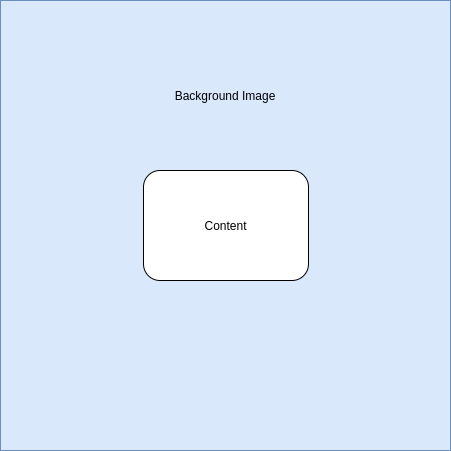
\includegraphics[scale=0.25]{./genderize-top-level}
  \caption{طراحی سطح بالا}
\end{figure}

\پاراگراف{}
مستطیل میانی تمامی محتویات قابل نمایش شما را می‌بایست شامل شود. این مستطیل می‌بایست تنها به اندازه محتویات باشد اما برای نمایش زیباتر آن از لایه‌گذاری\پانویس{padding} استفاده کنید.
محتوای شما از دو قسمت تشکیل شده است که به صورت افقی کنار یکدیگر قرار گرفته‌اند. قسمت اول یک فرم است که خود از دو ورودی تشکیل شده است. وروردی اول به شکل متنی بوده و کاربر اسم مورد نظر را وارد می‌کند.
ورودی دوم به شکل دو دکمه رادیویی است که به کاربر می‌کند اگر از پیش جواب را می‌داند آن را وارد کرده و این جواب برای آینده ذخیره می‌شود. در مورد جواب‌های ذخیره شده در ادامه بیشتر صحبت خواهد شد.
برای جایگذاری این اجزا مطابق آنچه آورده شده است \متن‌سیاه{می‌بایست} از \متن‌لاتین{flex} یا \متن‌لاتین{grid} استفاده کنید.

\begin{figure}[h]
  \centering
  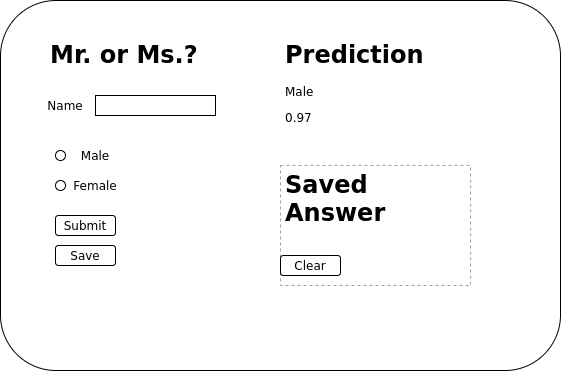
\includegraphics[scale=0.3]{./genderize-content}
  \caption{طراحی مستطیل محتوا}
\end{figure}

\پاراگراف{}
پس از پر کردن فرم کاربر گزینه درخواست\پانویس{submit} را زده و به این درخواست ایشان ارسال می‌شود. در مورد فرم ورود اطلاعات موارد زیر را مدنظر داشته باشید:

\شروع{فقرات}
\فقره اسمی که کاربر وارد می‌کند می‌بایست \متن‌سیاه{حداکثر} ۲۵۵ کاراکتر داشته باشد.
\فقره اسم وارد شده توسط کاربر می‌بایست فقط از فاصله، حروف بزرگ و کوچک انگلیسی تشکیل شده باشد.
\فقره دکمه \متن‌لاتین{submit} \متن‌سیاه{نباید} رفتار پیش‌فرض مرورگر را انجام بدهد.
\پایان{فقرات}

برای پیش‌بینی جنسیت اسم داده شده از وبگاه زیر استفاده می‌کنیم:

\begin{latin}\begin{center}
https://api.genderize.io/?name=hassan
\end{center}\end{latin}

شما نام را در قالب یک رشته تقاضا\پانویس{query string} و به صورت \متن‌لاتین{GET} برای این وبگاه ارسال می‌کنید و در نهایت حاصل پیش‌بینی را به کاربر نمایش می‌دهید. خروجی این درخواست به شکل زیر می‌باشد:

\begin{latin}
\begin{minted}[bgcolor=LightGray]{json}
{
  "name":"hassan",
  "gender":"male",
  "probability":0.97,
  "count":49197
}
\end{minted}
\end{latin}

در نظر داشته باشید که پاسخ در قالب \متن‌لاتین{json} است و شما \متن‌سیاه{می‌بایست} آن به یک \متن‌لاتین{object} در جاوااسکریپ تبدیل کنید.

\شروع{امتیازی}
ممکن است به دلیل شبکه ارسال درخواست به خطا بخورد یا اینکه این وبگاه نتواند برای یک نام پیش‌بینی داشته باشد (برای نمونه این وبگاه برای نام ``محمد حسین'' پیش‌بینی ندارد). شما می‌بایست این خطاها را با نمایش پیام خطا به کاربر رسیدگی کنید. دقت داشته باشید که نمایش می‌بایست در وبگاه شما صورت بگیرد و نمایش در کنسول مرورگر نمره‌ای دریافت نمی‌کند.
\پایان{امتیازی}

\زیرقسمت{جواب‌های ذخیره شده}
\پاراگراف{}
زمان‌هایی وجود دارد که وبگاه پیش‌بینی اشتباه انجام می‌دهد، در این صورت می‌توان با پرسش از دانشجو به پاسخ صحیح رسید. در این صورت این سامانه می‌بایست توانایی ذخیره کردن پاسخ صحیح را داشته باشد. برای ذخیره کردن پاسخ صحیح یک راه استفاده از کوکی‌ها و یک راه دیگر استفاده از \متن‌لاتین{local storage} می‌باشد.
در نهایت اگر اسم وارد شده در قالب کوکی یا کلیدی در \متن‌لاتین{local storage} موجود باشد شما می‌بایست پاسخ ذخیره شده را \متن‌سیاه{نیز} به کاربر نمایش دهید.
در صورتی که یک ذخیره‌سازی برای یک نام صورت گرفته باشد و کاربر دوباره از قسمت ذخیره‌سازی استفاده کند مقدار قبلی \متن‌سیاه{پاک} خواهد شد.
در صورتی که کاربر بخواهد مقدار ذخیره شده برای یک اسم را پاک کند، بعد از ارسال درخواست برای آن نام می‌تواند از دکمه پاک کردن که در قسمت جواب‌های ذخیره شده نمایش داده می‌شود استفاده کند. دقت داشته باشید که قسمت جواب‌های ذخیره شده
در صورت وجود جواب ذخیره شده به نمایش درخواهد آمد.

\زیرقسمت{گام به گام}

\پاراگراف{}
در این قسمت می‌خواهیم رویه کار با این وبگاه را یکبار به صورت گام به گام مرور کنیم.

\شروع{شمارش}
\فقره کاربر می‌خواهد جنسیت اسم ``حسن'' را پیدا کند.
\فقره کاربر اسم ``حسن'' را در قسمت مشخص شده وارد می‌کند و عملیات پیش‌بینی انجام می‌شود.
\فقره نتیجه پیش‌بینی به او نمایش داده می‌شود و می‌تواند در صورت لزوم آن را ذخیره کند.
\پایان{شمارش}

\شروع{شمارش}
\فقره کاربر می‌خواهد جنسیت اسم ``حسن'' را پیدا کند ولی پیش‌بینی میکند این اسم مردانه باشد.
\فقره کاربر اسم ``حسن'' را در قسمت مشخص شده وارد می‌کند و عملیات پیش‌بینی انجام می‌شود.
\فقره نتیجه پیش‌بینی به کاربر نمایش داده می‌شود ولی کاربر ترجیح می‌دهند از دانش خود استفاده کرده و جنسیت مردانه را برای این اسم ذخیره کند.
\پایان{شمارش}

\شروع{شمارش}
\فقره کاربر می‌خواهد جنسیت اسم ``حسن'' را پیدا کند اما پیشتر این اسم را وارد کرده و نتیجه آن را ذخیره کرده است.
\فقره کاربر اسم ``حسن'' را در قسمت مشخص شده وارد می‌کند و عملیات پیش‌بینی انجام می‌شود.
\فقره نتیجه پیش‌بینی به کاربر نمایش داده می‌شود، در کنار آن قید می‌شود که نتیجه از پیش برای این اسم ذخیره شده است.
\فقره کاربر می‌تواند نتیجه ذخیره شده را تغییر داده یا آن را حذف نماید.
\پایان{شمارش}

\شروع{شمارش}
\فقره کاربر می‌خواهد جنسیت اسم ``حسن'' را پیدا کند اما پیشتر این اسم را وارد کرده و نتیجه مورد نظر خود را ذخیره کرده است.
\فقره کاربر اسم ``حسن'' را در قسمت مشخص شده وارد می‌کند و عملیات پیش‌بینی انجام می‌شود.
\فقره نتیجه پیش‌بینی به کاربر نمایش داده می‌شود، در کنار آن قید می‌شود که نتیجه از پیش برای این اسم ذخیره شده است.
\فقره کاربر می‌تواند نتیجه ذخیره شده را تغییر داده یا آن را حذف نماید.
\پایان{شمارش}

\زیرقسمت{انتشار}
\پاراگراف{}
پیاده‌سازی یک وب‌سایت بدون قرار دادن آن برای همه، کار کاملی نخواهد بود. از این رو در قسمت نحوه انتشار این وبگاه روی \تارنما{https://github.com}{گیت‌هاب} را مرور می‌کنیم.

در گام اول می‌بایست یک مخزن ایجاد کرده و کد خود را در آن قرار دهید. فایل \متن‌لاتین{index.html} با همین نام می‌بایست در ریشه\پانویس{root} مخزن شما قرار داشته باشد.
در فایل \متن‌لاتین{index.html} می‌توانید به صورت نسبی\پانویس{relative} سایر فایل‌ها مانند عکس یا اسکریپت‌ها و \نقاط‌خ را ارجاع دهید.

در گام بعد می‌بایست از نوار بالا به زبانه \متن‌لاتین{settings} رفته و از منوی سمت چپ گزینه \متن‌لاتین{pages} را انتخاب کنید.
در قسمت \متن‌لاتین{pages} گزینه \متن‌لاتین{None} را انتخاب کرده و آن را به نام شاخه\پانویس{branch} خود تغییر دهید.

\begin{figure}[h]
  \centering
  \includegraphics[scale=0.3]{./github-step-1}
  \caption{زبانه \متن‌لاتین{settings}}
\end{figure}

\begin{figure}[h]
  \centering
  \includegraphics[scale=0.3]{./github-step-2}
  \caption{قسمت \متن‌لاتین{pages} در زبانه \متن‌لاتین{settings}}
\end{figure}

بعد از این وب‌سایت شما از آدرس زیر قابل رویت خواهد بود.

\begin{latin}\begin{center}
https://<username>.github.io/<repo>
\end{center}\end{latin}

که در آن \متن‌لاتین{username} نام کاربری شما در گیت‌هاب و \متن‌لاتین{repo} نام مخزن شماست. این آدرس در قابل یک فایل متنی در کنار سایر موارد پروژه خود بارگذاری نمایید.

\زیرقسمت{نکات پیاده‌سازی}

\شروع{فقرات}
\فقره برای کدهایتان از کامنت استفاده کنید. توضیح کارکرد بلاک‌های \متن‌لاتین{CSS} اجباری می‌باشد. توابعی و قطعات کد جاوا اسکریپت نیز می‌بایست حداقل یک خط کامنت داشته باشند.
\فقره کامنت فارسی یا انگلیسی موردی ندارد اما از فینگلیش (!) نوشتن پرهیز کنید.
\فقره استفاده از کتابخانه‌ها و چهارچوب‌ها در پروژه مجاز \متن‌سیاه{نمی‌باشد}.
\فقره از آنجایی که این پروژه در قالب \متن‌سیاه{امتحان میانترم} می‌باشد از تغییر دادن صورت مساله یا انجام موارد خارج از موارد مطرح شده خودداری کنید.
\پایان{فقرات}

\زیرقسمت{تحویل‌دادنی‌ها}

\شروع{فقرات}
\فقره کد و وابستگی‌های مربوط به وب‌گاه که برای بالا آوردن آن لازم است، شامل \متن‌لاتین{HTML}، \متن‌لاتین{CSS}، \متن‌لاتین{Javascript}، عکس، فونت و \نقاط‌خ
\فقره یک فایل متنی که آدرس مخزن شما در گیت‌هاب می‌باشد و سایت برای فعال و قابل دسترس است.
\فقره شما می‌بایست در مخزن گیت‌هاب داده شده با اکانت خودتان \متن‌لاتین{commit} داشته باشید.
\پایان{فقرات}

\زیرقسمت{پرسش‌های متداول}

صورت پروژه در مهلت انجام پروژه بر پایه سوالات شما به روزرسانی خواهد شد.
\شروع{توضیح}
\فقره[پرسش (۱)] اگر کاربر دو دیتای متفاوت برای یک اسم ذخیره کند تکلیف چیست؟
\فقره[پاسخ] آخرین مقدار بر روی مقدارهای قبلی ذخیره می‌شود.
\فقره[پرسش (۲)] عکس پس‌زمینه خاصی مدنظر است؟ اگر نیست قرار دادن آن اجباری است؟ \متن‌لاتین{CSS} خاصی باید داشته باشد؟
\فقره[پاسخ] خیر عکس خاصی مدنظر نیست، اما قرار دادن عکس اجباری می‌باشد. دقت داشته باشید که این عکس می‌بایست تمام پس‌زمینه را پوشانده باشد و در صفحه‌های نمایش متفاوت نمایش صحیح داشته باشد. لازم به ذکر است نیازی نیست وبگاه شما قابل نمایش در گوشی‌های موبایل و \نقاط باشد بلکه تنها کافی است در صفحات نمایش دسکتاپ به صورت مناسب نمایش داده شود.
\فقره[پرسش (۳)] اگر کاربر جنسیت رو مشخص کند، درخواست نباید ارسال شود؟
\فقره[پاسخ] درخواست می‌بایست همیشه ارسال شود تا بتوان آنچه کاربر ذخیره کرده یا می‌کند با پیش‌بینی سایت مطابقت داد.
\فقره[پرسش (۴)] آیا استفاده از کتابخانه‌ی \متن‌لاتین{bootstrap} مجاز است؟
\فقره[پاسخ] خیر مجاز \متن‌سیاه{نمی‌باشد}.
\فقره[پرسش (۵)] برای قسمت امتیازی که گفته شده است نمایش خطاها در وبگاه صورت بگیرد، اینکه صرفا یک \متن‌لاتین{alert} بدهد مورد قبول است؟
\فقره[پاسخ] خیر، نمایش می‌بایست در قالب ارائه یک متن در داخل وب‌گاه صورت بپذیرد و استفاده از \متن‌لاتین{alert} و \متن‌لاتین{confirm} مجاز نمی‌باشد.
\فقره[پرسش (۶)] آیا برای نمایش خطاها در صفحه، تغییر شِما ایرادی ندارد؟
\فقره[پاسخ] خیر برای این قسمت \متن‌سیاه{امتیازی} می‌توانید مقداری تغییر داشته باشید.
\فقره[پرسش (۷)] آیا انجام قسمت انتشار روی گیت‌هاب اجباری است؟
\فقره[پاسخ] بله شما در تمرین اول با نحوه کار با گیت آشنا شدید بنابراین انجام این قسمت اجباری است.
\فقره[پرسش (۷)] آیا استفاده از \متن‌لاتین{flex} یا \متن‌لاتین{grid} اجباری است؟
\فقره[پاسخ] بله، شما می‌بایست برای قراردادن اشیا از یکی از این دو راه استفاده کنید.
\پایان{توضیح}

\end{document}
